
\documentclass[10pt,openany,a4paper]{article}
\usepackage{tikz, pgfplots, tkz-euclide,calc}
\usetikzlibrary{patterns,shapes.arrows,calc}
\usepackage{fancyhdr}
\usepackage{enumerate,enumitem}
\usepackage{cancel}
\usepackage{varwidth}

% TAMBAHKAN PACKAGE SENDIRI KALAU KURANG

\usepackage{geometry}
\geometry{
	left = 22mm,
	right = 22mm,
	top = 25mm,
	bottom = 25mm,
}
\usepackage{graphicx}
\usepackage{subcaption}
\usepackage{soul}
\usepackage{hyperref}
\usepackage{float}
\usepackage{setspace}
\usepackage{afterpage}
\usepackage{xcolor}
\usepackage[nosectionbib]{apacite}
\usepackage{lmodern}
\usepackage{mathtools}
\usepackage{upgreek}
\usepackage{siunitx}
% \usepackage{fontawesome5}
\usepackage{fontawesome6}
\usepackage{physics}
\usepackage{pdfpages}
\usepackage{hyperref}
\renewcommand{\baselinestretch}{1.3}
\usepackage{multicol}
\usepackage{hyperref,ragged2e,amsmath,multicol,gensymb,setspace,
fancyhdr,amsfonts,tikz,pgfplots,nccmath,enumerate,verbatim,amsthm,physics}
\usepgfplotslibrary{polar,fillbetween}
% Disable tikz externalization to avoid requiring -shell-escape
\usepgfplotslibrary{external}
\tikzexternalize[prefix=tikz/]
\tikzset{reuse path/.code={\pgfsyssoftpath@setcurrentpath{#1}}}
\usetikzlibrary{shapes.geometric,arrows}
\newcommand\mylog[1]{\mathop{{}^{#1}\mathrm{log}}}
\pgfplotsset{compat=1.15}
\pgfplotsset{my style/.append style={axis x line=middle, axis y line=
middle, xlabel={$x$}, ylabel={$y$}, axis equal }}
\usepackage{etoolbox}
% remove stray \makeatother
\newtheorem{defn}{Definisi}[section]
\newtheorem{teo}[defn]{Teorema}
\newtheorem{thm}{Teorema}[section]
\newtheorem{lemma}{Lemma}
\newtheorem{lemmas}[defn]{Lemma}
\newtheorem{cor}[defn]{Akibat}
\newtheorem{asumsi}[defn]{Asumsi}
\theoremstyle{definition}
\newtheorem{con}{Contoh}[section]
\theoremstyle{definition}
\theoremstyle{plain}
\newtheorem{prop}{Proposisi}[section]
\renewcommand{\proofname}{Bukti}
\renewcommand{\thethm}{\arabic{chapter}.\arabic{thm}}

\newcommand{\normlp}[1]{\left\|#1\right\|_{L^p_{\lambda}(0,T;H)}}% Fungsi norm (||x||)
\newcommand{\R}{\mathbb{R}}
\renewcommand{\natural}{\mathbb{N}}
\newcommand{\Xpl}{X^R_{p,\lambda}}
\newcommand{\Xpls}{X^R_{p,\lambda^*}}
\newcommand{\qpl}{q^R_{p,\lambda}}
\newcommand{\qpls}{q^R_{p,\lambda^*}}
\pagestyle{fancy}
\fancyhf{}
\lhead{Halaman \thepage}
% \cfoot{\faXTwitter\ \href{https://x.com/ahmadzakiyudin_/}{@ahmadzakiyudin\_} | \faInstagram\ \href{https://instagram.com/ahmadzakiyudin_/}{@ahmadzakiyudin\_} | \faTiktok\ \href{https://tiktok.com/@ahmathz/}{@ahmathz}}
% \rhead{Pembahasan Soal ETS \\ Kalkulus 1 ITS 2025/2026}
\hypersetup{
    colorlinks=true,
    linkcolor=blue,
    filecolor=blue,      
    urlcolor=blue,
}
\newenvironment{jawab}[2][tes]{
% \fbox{\begin{minipage}{14.65cm}
\textbf{Kata kunci materi:} #1.\\
\textbf{Penyelesaian:} #2
% \end{minipage}}
}{}

\newenvironment{jawab2}[2][tes]{
\fbox{\begin{minipage}{14.65cm}
 #2
\end{minipage}}}{}

\newenvironment{jawaban}[2][tes]{
\colorlet{oldcolor}{.}
        \color{red}
        \setlength{\fboxrule}{1pt}\boxed{\color{oldcolor}#2}\color{oldcolor}.
}{}

\newenvironment{jawaban2}[2][tes]{
\colorlet{oldcolor}{.}
        \color{red}
        \setlength{\fboxrule}{1pt}\fbox{\color{oldcolor}#2}\color{oldcolor}.
}{}

\newenvironment{penting}[2][tes]{
\colorlet{oldcolor}{.}
\color{blue}
\fbox{\color{oldcolor}#2}\color{oldcolor}
}{}

\begin{document}
% \begin{titlepage}
%     \vspace*{\fill}
%     \begin{center}
%       \Huge {PEMBAHASAN SOAL EAS \\ KALKULUS II \\ TAHUN 2024/2025}\\[0.4 cm]
%       \huge {Ahmad Hisbu Zakiyudin}\\[0.2 cm]
%       \Large {(\href{https://instagram.com/ahmadzakiyudin_/}{@ahmadzakiyudin\_})}
%     \end{center}
%     \vspace*{\fill}
%   \end{titlepage}
% !TEX root = ../../BookTemplate.tex
%%%%%%%%%%%%%%%%%%%%%%%%%%%%%%%%%%%%%%%%%%%%%%%%%%%%%%%%%%%%%%%%%%%%%%%%%%%%%%%%%%
% \begin{titlepage}
%     \raggedleft	
% 	\hspace{.025\textwidth}
% 	\parbox[b]{\textwidth}{
%     \vspace{1.5cm}
% 		{\Huge\bfseries Pembahasan Soal EAS}                \\[20pt]
% 		{\huge\textit\ Kalkulus II}\\ \\[10pt]
%         {\Large\textsc{Tahun 2024/2025}}}
% \vfill
% \rule{1pt}{.14\textheight}
% \hspace{.025\textwidth}
%     \raisebox{10pt}{\parbox[b]{.95\textwidth}{ 
%         {\Large\textsc{Ahmad Hisbu Zakiyudin}}              \\[10pt]
%         \large{\href{https://instagram.com/ahmadzakiyudin_/}{@ahmadzakiyudin\_}}               \\[25pt]
%         {\large 5 Juni 2026}}}
% \end{titlepage}
\begin{titlepage}
	\centering % Center everything on the title page
	% \scshape % Use small caps for all text on the title page
	\vspace*{1.5\baselineskip} % White space at the top of the page
% ===================
%	Title Section 	
% ===================

	\rule{13cm}{1.6pt}\vspace*{-\baselineskip}\vspace*{2pt} % Thick horizontal rule
	\rule{13cm}{0.4pt} % Thin horizontal rule
	
		\vspace{0.75\baselineskip} % Whitespace above the title
% ========== Title ===============	
	{	\Huge Soal Tryout ETS\\ 
			\vspace{4mm}
		Kalkulus 1 \\ \vspace{2mm} \huge{Tahun 2026/2027}\\ \vspace{2mm} \Large{(Paket 3)}\\	}
% ======================================
		\vspace{0.75\baselineskip} % Whitespace below the title
	\rule{13cm}{0.4pt}\vspace*{-\baselineskip}\vspace{3.2pt} % Thin horizontal rule
	\rule{13cm}{1.6pt} % Thick horizontal rule
	
		\vspace{1.75\baselineskip} % Whitespace after the title block
% =================
%	Information	
% =================
{\large Oleh: Ahmad Hisbu Zakiyudin}
	% {\large Oleh: Ahmad Hisbu Zakiyudin \\
	% 	\vspace*{1.2\baselineskip}
	% \href{https://instagram.com/ahmadzakiyudin_/}{@ahmadzakiyudin\_}} \\
	\vfill
	\vspace{1mm}
\huge{Selamat Belajar!}
\end{titlepage}
\makeatletter
\setlength\fboxsep{3pt}
% ensure enough header height for fancyhdr
\setlength{\headheight}{24pt}
% Kop tiap kelompok: #1 kelompok, #2 kelas, #3 departemen, #4 jadwal kuliah, #5 sesi
\newcommand{\kopsoal}[5]{%
 \begin{center}
	{\underline{\textbf{\MakeUppercase{Tryout ETS Kalkulus 1 Tahun 2026/2027}}}}
    \end{center}

    \begin{center}
	\begin{tabular}{lcl}
		Mata kuliah/SKS & : & Kalkulus 1 ( SM234101 ) / 3 SKS\\
		Kelompok & : & #1\\
		Kelas & : & #2\\
		Departemen & : & #3\\
		Jadwal kuliah & : & #4\\
		Sesi & : & #5\\
		Waktu & : & 100 menit\\
		Sifat & : & Tertutup\\
  ~
	\end{tabular}

    \noindent\rule{\textwidth}{2.pt}
        \end{center}}

% Kop kelompok IUP (bahasa Inggris): #1 kelompok, #2 kelas, #3 departemen, #4 jadwal kuliah, #5 sesi
\newcommand{\kopsoaliup}[5]{%
 \begin{center}
	{\underline{\textbf{\MakeUppercase{Tryout ETS Kalkulus 1 Tahun 2026/2027}}}}
    \end{center}

    \begin{center}
	\begin{tabular}{lcl}
		Course / Credit & : & Kalkulus 1 ( SM234101 ) / 3 SKS\\
		Group & : & #1\\
		Class & : & #2\\
		Department & : & #3\\
		Lecture schedule & : & #4\\
		Session & : & #5\\
		Time & : & 100 minutes\\
		Type & : & Closed\\
  ~
	\end{tabular}

    \noindent\rule{\textwidth}{2.pt}
        \end{center}}

% Kop tryout Matematika 2 SKS: #1 kelompok, #2 kelas, #3 departemen, #4 jadwal kuliah, #5 sesi
\newcommand{\kopsoalmat}[5]{%
 \begin{center}
	{\underline{\textbf{\MakeUppercase{Tryout ETS Matematika Tahun 2026/2027}}}}
    \end{center}

    \begin{center}
	\begin{tabular}{lcl}
		Mata kuliah/SKS & : & Matematika ( SM234152 ) / 2 SKS\\
		Kelompok & : & #1\\
		Kelas & : & #2\\
		Departemen & : & #3\\
		Jadwal kuliah & : & #4\\
		Sesi & : & #5\\
		Waktu & : & 100 menit\\
		Sifat & : & Tertutup\\
  ~
	\end{tabular}

    \noindent\rule{\textwidth}{2.pt}
        \end{center}}

% Kop tryout Matematika 2 SKS IUP (bahasa Inggris)
\newcommand{\kopsoalmatiup}[5]{%
 \begin{center}
	{\underline{\textbf{\MakeUppercase{Tryout ETS Matematika Tahun 2026/2027}}}}
    \end{center}

    \begin{center}
	\begin{tabular}{lcl}
		Course / Credit & : & Matematika ( SM234152 ) / 2 SKS\\
		Group & : & #1\\
		Class & : & #2\\
		Department & : & #3\\
		Lecture schedule & : & #4\\
		Session & : & #5\\
		Time & : & 100 minutes\\
		Type & : & Closed\\
  ~
	\end{tabular}

    \noindent\rule{\textwidth}{2.pt}
        \end{center}}

%%%%%%%%%%%%%%%%%%%%%%%%%%%%%%%%%%%%%%%%%%%%%%%%%%%%%%%%%%%%%%%%%%%%%%%%%%%%%%
% Kal-5 | Paket 3: subbab per nomor 1.1, 2.3, 2.4, 3.3, 4.2
% Kisi-kisi hari Senin: subbab 1.1, 1.5, 2.3, 2.4, 3.1, 3.3, 4.2, 4.4
\kopsoal{Kal-5}{22-27}{T. Fisika, T. Material dan Metalurgi, Rkp}{Senin, Rabu; 07.00-09.30}{1}
\begin{enumerate}
    \item \textbf{[Subbab 1.1]} Tentukan semua nilai $x$ yang memenuhi
    \begin{align*}
        \frac{x^2-2x-3}{x+2}\leq 0.
    \end{align*}

    \item \textbf{[Subbab 2.3]} Grafik fungsi $y=f(x)$ dengan domain $[-3,3]$ diberikan pada gambar berikut.
    \begin{center}
        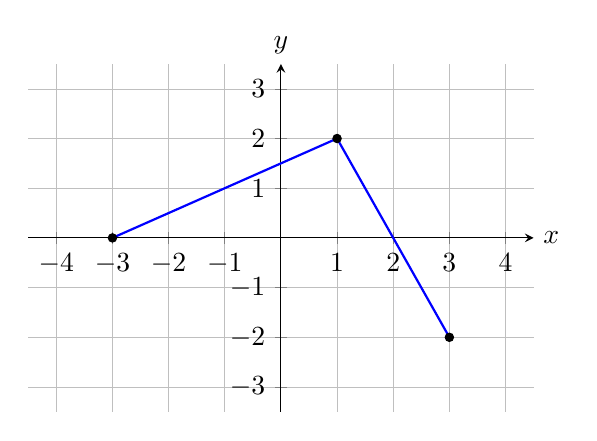
\begin{tikzpicture}
            \begin{axis}[
        axis lines = middle,
        xlabel = $x$,
        ylabel = {$y$},
        grid=both,
        grid style={line width=.1pt, draw=gray!10},
        major grid style={line width=.2pt,draw=gray!50},
        x label style={anchor=west}, % label x ke kanan
        y label style={anchor=south}, % label y ke atas
        samples=200,
        legend style={
                at={(1.1,1)},
                anchor=north west,
                font=\small,         % mengecilkan ukuran font
                row sep=1pt,         % jarak antar baris legend
                inner sep=1pt,       % margin dalam kotak legend
                nodes={scale=0.7}    % skalakan isi legend
            },
        xtick={-4,-3,...,4},
        ytick={-3,-2,...,3},
        xmin=-4.5, xmax=4.5,
        ymin=-3.5, ymax=3.5,
        width=8cm,
        height=6cm
    ]
\addplot[color=blue, thick] coordinates {(-3,0) (1,2) (3,-2)};
\draw[fill=black] (-3,0) circle (1.5pt);
\draw[fill=black] (1,2) circle (1.5pt);
\draw[fill=black] (3,-2) circle (1.5pt);
\end{axis}
        \end{tikzpicture}
    \end{center}
    \begin{enumerate}
        \item Tentukan domain dan range dari $f$.
        \item Gambarkan sketsa grafik $y=f(x+1)-2$ (jelaskan pergeserannya).
    \end{enumerate}

    \item \textbf{[Subbab 2.4]} Diberikan fungsi $f(x)=1+\sqrt{2x-4}$.
    \begin{enumerate}
        \item Tentukan domain dan range dari $f$.
        \item Dapatkan $f^{-1}(x)$ beserta domainnya.
    \end{enumerate}

    \item \textbf{[Subbab 3.3]} Tentukan nilai $a>0$ sehingga $\displaystyle\lim_{x\to+\infty}\frac{\sqrt{ax^2+3}}{2x-1}=3$.

    \item \textbf{[Subbab 4.2]} Diketahui
    \begin{align*}
        \lim_{h\to 0}\frac{(2+h)^3-8}{h}
    \end{align*}
    menyatakan turunan suatu fungsi $f$ di suatu titik $x=a$. Tentukan $f$ dan $a$, kemudian hitung nilai limit tersebut.
\end{enumerate}

\newpage

%%%%%%%%%%%%%%%%%%%%%%%%%%%%%%%%%%%%%%%%%%%%%%%%%%%%%%%%%%%%%%%%%%%%%%%%%%%%%%
% Kal-6 | Paket 3: subbab per nomor 1.1, 2.3, 2.4, 3.3, 4.2
% Kisi-kisi hari Senin: subbab 1.1, 1.5, 2.3, 2.4, 3.1, 3.3, 4.2, 4.4
\kopsoal{Kal-6}{28-31}{T. Perkapalan, T. Transportasi Laut, T. Bangunan Lepas Pantai}{Senin, Rabu; 07.00-09.30}{1}
\begin{enumerate}
    \item \textbf{[Subbab 1.1]} Selesaikan pertidaksamaan berikut
    \begin{align*}
        \frac{(x-1)(x+2)^2}{x-3}\leq 0.
    \end{align*}

    \item \textbf{[Subbab 2.3]} Gunakan kurva dasar $y=x^2$ serta sifat pencerminan dan translasi untuk menggambar sketsa grafik $y=3-(x-2)^2$. Tandai titik puncak dan titik potongnya dengan sumbu-sumbu koordinat. (Jelaskan prosesnya.)

    \item \textbf{[Subbab 2.4]} Diberikan fungsi $f(x)=2x^2-8x+5$ dengan $x\geq 2$.
    \begin{enumerate}
        \item Tentukan range dari $f$.
        \item Dapatkan $f^{-1}(x)$ beserta domainnya.
    \end{enumerate}

    \item \textbf{[Subbab 3.3]} Hitunglah $\displaystyle\lim_{x\to-\infty}\frac{2x^3-x+1}{4-x^3}$.

    \item \textbf{[Subbab 4.2]} Tentukan nilai $a$ dan $b$ agar fungsi
    \begin{align*}
        f(x)=\begin{cases}
            x^2+x, & x\leq 2\\
            ax+b, & x>2
        \end{cases}
    \end{align*}
    kontinu dan dapat diturunkan di $x=2$.
\end{enumerate}

\newpage

%%%%%%%%%%%%%%%%%%%%%%%%%%%%%%%%%%%%%%%%%%%%%%%%%%%%%%%%%%%%%%%%%%%%%%%%%%%%%%
% Kal-iup-1 | Paket 3: subbab per nomor 1.1, 2.3, 2.4, 3.1, 4.2
% Kisi-kisi hari Senin: subbab 1.1, 1.5, 2.3, 2.4, 3.1, 3.3, 4.2, 4.4
\kopsoaliup{Kal-iup-1}{61, 68}{Chemical, Environmental, Electrical Engineering}{Monday, Wednesday; 07.00-09.30}{1}
\begin{enumerate}
    \item \textbf{[Subbab 1.1]} Solve the following inequality.
    \begin{align*}
        \frac{2x}{x+1}\geq x.
    \end{align*}

    \item \textbf{[Subbab 2.3]} Sketch the base curve $y=\dfrac{1}{x}$. Based on that base curve, use translation to sketch the curve $y=\dfrac{1}{x+3}-2$. (Explain the process).

    \item \textbf{[Subbab 2.4]} Given a function $f(x)=3-\sqrt{x-2}$. Determine:
    \begin{enumerate}
        \item[a)] The domain and range of $f$;
        \item[b)] $f^{-1}(x)$ and its domain;
        \item[c)] Sketch the graph of $f(x)$ and $f^{-1}(x)$ in the same coordinate plane.
    \end{enumerate}

    \item \textbf{[Subbab 3.1]} The graph of a function $f$ is given below.
    \begin{center}
        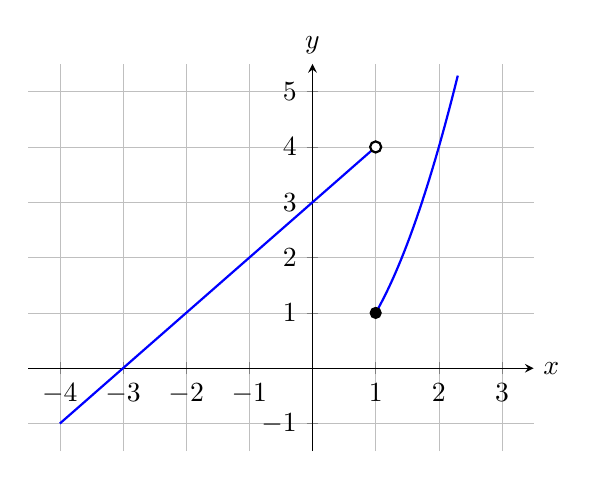
\begin{tikzpicture}
            \begin{axis}[
        axis lines = middle,
        xlabel = $x$,
        ylabel = {$y$},
        grid=both,
        grid style={line width=.1pt, draw=gray!10},
        major grid style={line width=.2pt,draw=gray!50},
        x label style={anchor=west}, % label x ke kanan
        y label style={anchor=south}, % label y ke atas
        samples=200,
        legend style={
                at={(1.1,1)},
                anchor=north west,
                font=\small,         % mengecilkan ukuran font
                row sep=1pt,         % jarak antar baris legend
                inner sep=1pt,       % margin dalam kotak legend
                nodes={scale=0.7}    % skalakan isi legend
            },
        xtick={-4,-3,...,3},
        ytick={-1,0,...,5},
        xmin=-4.5, xmax=3.5,
        ymin=-1.5, ymax=5.5,
        width=8cm,
        height=6.5cm
    ]
\addplot[domain=-4:1, color=blue, thick, samples=2] {x+3};
\addplot[domain=1:2.3, color=blue, thick] {x^2};
\draw[fill=white, thick] (1,4) circle (2pt);
\draw[fill=black] (1,1) circle (2pt);
\end{axis}
        \end{tikzpicture}
    \end{center}
    Find:
    \begin{enumerate}
        \item[a.] $\displaystyle\lim_{x\to 1^-}f(x)$, $\displaystyle\lim_{x\to 1^+}f(x)$, $\displaystyle\lim_{x\to 1}f(x)$, and $f(1)$;
        \item[b.] $\displaystyle\lim_{x\to -1}f(x)$ and $\displaystyle\lim_{x\to 2}f(x)$.
    \end{enumerate}

    \item \textbf{[Subbab 4.2]} Show that $f(x)=|x-2|$ is continuous at $x=2$ but not differentiable at $x=2$.
\end{enumerate}

\newpage

%%%%%%%%%%%%%%%%%%%%%%%%%%%%%%%%%%%%%%%%%%%%%%%%%%%%%%%%%%%%%%%%%%%%%%%%%%%%%%
% Kal-iup-4 | Paket 3: subbab per nomor 1.1, 2.3, 2.4, 3.1, 4.2
% Kisi-kisi hari Senin: subbab 1.1, 1.5, 2.3, 2.4, 3.1, 3.3, 4.2, 4.4
\kopsoaliup{Kal-iup-4}{65, 66, 67}{Statistics, Marine Engineering (JD), Informatics}{Monday, Wednesday; 07.00-09.30}{1}
\begin{enumerate}
    \item \textbf{[Subbab 1.1]} Solve the following inequality.
    \begin{align*}
        \frac{x+3}{x-2}\geq 3.
    \end{align*}

    \item \textbf{[Subbab 2.3]} Sketch the graph of $y=|x|$. Then, use reflection and translation to sketch the graph of $y=3-|x+1|$ and determine its highest point.

    \item \textbf{[Subbab 2.4]} Given a function $f(x)=\dfrac{1}{x+2}-1$. Determine:
    \begin{enumerate}
        \item[a)] The domain and range of $f$;
        \item[b)] $f^{-1}(x)$ and its domain.
    \end{enumerate}

    \item \textbf{[Subbab 3.1]} Given $f(x)=\begin{cases}
        x^2-1, & x<2\\
        2x+k, & x\geq 2
    \end{cases}$.\\
    Find the value of $k$ such that $\displaystyle\lim_{x\to 2}f(x)$ exists. Then, sketch the graph of $f$ for that value of $k$.

    \item \textbf{[Subbab 4.2]}
    \begin{enumerate}
        \item[a.] Suppose that $f(3)=-1$ and $f'(3)=3$. Find the equation of the tangent line to the curve $y=f(x)$ at $x=3$.
        \item[b.] Verify, using the definition of derivative, that $f(x)=x^2-3x-1$ satisfies $f(3)=-1$ and $f'(3)=3$.
    \end{enumerate}
\end{enumerate}

\newpage

%%%%%%%%%%%%%%%%%%%%%%%%%%%%%%%%%%%%%%%%%%%%%%%%%%%%%%%%%%%%%%%%%%%%%%%%%%%%%%
% Kal-9 | Paket 3: subbab per nomor 1.1, 2.3, 2.4, 3.1, 4.2
% Kisi-kisi hari Senin: subbab 1.1, 1.5, 2.3, 2.4, 3.1, 3.3, 4.2, 4.4
\kopsoal{Kal-9}{44-48}{T. Sistem Perkapalan, T. Kelautan, T. Komputer}{Senin, Rabu; 12.30-15.00}{3}
\begin{enumerate}
    \item \textbf{[Subbab 1.1]} Dapatkan himpunan penyelesaian pertidaksamaan
    \begin{align*}
        \frac{x^2-5x+6}{x^2-1}\leq 0.
    \end{align*}

    \item \textbf{[Subbab 2.3]} Diberikan $f(x)=4-x^2$. Gambarkan sketsa grafik
    \begin{align*}
        y=\frac{1}{2}\big(f(x)+|f(x)|\big).
    \end{align*}
    (Petunjuk: tinjau kasus $f(x)\geq 0$ dan $f(x)<0$.)

    \item \textbf{[Subbab 2.4]} Diberikan fungsi $f(x)=x^2+2x+3$ dengan $x\geq -1$.
    \begin{enumerate}
        \item Tentukan range dari $f$.
        \item Dapatkan $f^{-1}(x)$ beserta domainnya.
        \item Sketsa grafik $f(x)$ dan $f^{-1}(x)$ pada satu bidang koordinat.
    \end{enumerate}

    \item \textbf{[Subbab 3.1]} Buatlah sketsa grafik suatu fungsi $f$ yang memenuhi semua syarat berikut (banyak jawaban yang mungkin):
    \begin{enumerate}
        \item domain $f$ adalah $[-2,3]$,
        \item $f(-2)=0$, $f(0)=2$, dan $f(2)=1$,
        \item $\displaystyle\lim_{x\to 0^-}f(x)=1$, $\displaystyle\lim_{x\to 0^+}f(x)=-1$, dan $\displaystyle\lim_{x\to 2}f(x)=3$.
    \end{enumerate}

    \item \textbf{[Subbab 4.2]} Posisi sebuah partikel yang bergerak pada garis lurus pada saat $t$ detik adalah $s(t)=t^2-4t+1$ meter.
    \begin{enumerate}
        \item Tentukan kecepatan rata-rata partikel pada selang waktu $[1,3]$.
        \item Dengan menggunakan definisi turunan, tentukan kecepatan sesaat partikel pada saat $t=3$.
    \end{enumerate}
\end{enumerate}

\newpage

%%%%%%%%%%%%%%%%%%%%%%%%%%%%%%%%%%%%%%%%%%%%%%%%%%%%%%%%%%%%%%%%%%%%%%%%%%%%%%
% Kal-11 | Paket 3: subbab per nomor 1.1, 2.3, 2.4, 3.3, 4.2
% Kisi-kisi hari Senin: subbab 1.1, 1.5, 2.3, 2.4, 3.1, 3.3, 4.2, 4.4
\kopsoal{Kal-11}{51-54}{Biologi, Bioteknologi, Teknologi Informasi}{Senin, Rabu; 12.30-15.00}{3}
\begin{enumerate}
    \item \textbf{[Subbab 1.1]} Tentukan semua nilai $x$ yang memenuhi
    \begin{align*}
        \frac{1}{x+1}+\frac{1}{x-1}\geq 0.
    \end{align*}

    \item \textbf{[Subbab 2.3]} Grafik fungsi $y=f(x)$ dengan domain $[-3,4]$ terdiri dari dua ruas garis seperti pada gambar berikut.
    \begin{center}
        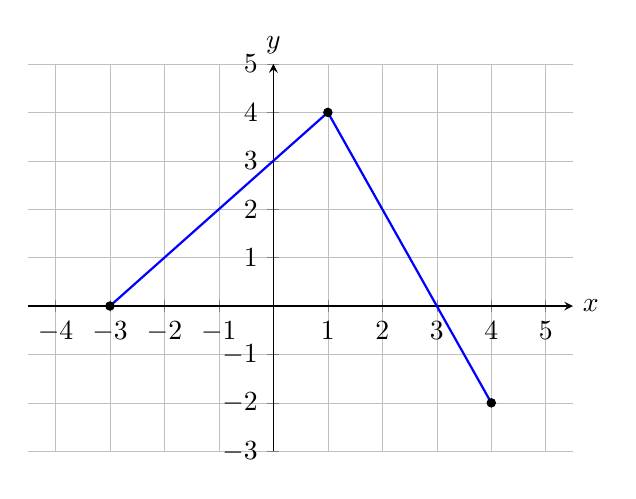
\begin{tikzpicture}
            \begin{axis}[
        axis lines = middle,
        xlabel = $x$,
        ylabel = {$y$},
        grid=both,
        grid style={line width=.1pt, draw=gray!10},
        major grid style={line width=.2pt,draw=gray!50},
        x label style={anchor=west}, % label x ke kanan
        y label style={anchor=south}, % label y ke atas
        samples=200,
        legend style={
                at={(1.1,1)},
                anchor=north west,
                font=\small,         % mengecilkan ukuran font
                row sep=1pt,         % jarak antar baris legend
                inner sep=1pt,       % margin dalam kotak legend
                nodes={scale=0.7}    % skalakan isi legend
            },
        xtick={-4,-3,...,5},
        ytick={-3,-2,...,5},
        xmin=-4.5, xmax=5.5,
        ymin=-3, ymax=5,
        width=8.5cm,
        height=6.5cm
    ]
\addplot[color=blue, thick] coordinates {(-3,0) (1,4) (4,-2)};
\draw[fill=black] (-3,0) circle (1.5pt);
\draw[fill=black] (1,4) circle (1.5pt);
\draw[fill=black] (4,-2) circle (1.5pt);
\end{axis}
        \end{tikzpicture}
    \end{center}
    Tentukan rumus $f(x)$ sebagai fungsi sepotong-sepotong, kemudian tentukan semua $x$ yang memenuhi $f(x)\geq 1$.

    \item \textbf{[Subbab 2.4]} Diberikan fungsi $f(x)=\dfrac{x+4}{2x-1}$.
    \begin{enumerate}
        \item Tentukan domain dan range dari $f$.
        \item Dapatkan $f^{-1}(x)$, kemudian tunjukkan bahwa $f^{-1}(x)=f(x)$.
    \end{enumerate}

    \item \textbf{[Subbab 3.3]} Hitunglah $\displaystyle\lim_{x\to+\infty}\left(\sqrt{9x^2+x}-3x\right)$.

    \item \textbf{[Subbab 4.2]} Tunjukkan bahwa $f(x)=x|x|$ dapat diturunkan di $x=0$ dan tentukan $f'(0)$.
\end{enumerate}

\newpage

%%%%%%%%%%%%%%%%%%%%%%%%%%%%%%%%%%%%%%%%%%%%%%%%%%%%%%%%%%%%%%%%%%%%%%%%%%%%%%
% Kal-12 | Paket 3: subbab per nomor 1.1, 2.3, 2.4, 3.1, 4.2
% Kisi-kisi hari Senin: subbab 1.1, 1.5, 2.3, 2.4, 3.1, 3.3, 4.2, 4.4
\kopsoal{Kal-12}{55-60}{Aktuaria, Teknik Informatika, RPL, RKA}{Senin, Rabu; 12.30-15.00}{3}
\begin{enumerate}
    \item \textbf{[Subbab 1.1]} Tentukan penyelesaian dari pertidaksamaan
    \begin{align*}
        \frac{x^2+2}{x+1}\geq 2.
    \end{align*}

    \item \textbf{[Subbab 2.3]} Gunakan kurva dasar $y=\sqrt[3]{x}$ serta sifat pencerminan dan translasi untuk menggambar sketsa grafik $y=-\sqrt[3]{x+1}$. (Jelaskan prosesnya.)

    \item \textbf{[Subbab 2.4]} Diberikan fungsi $f(x)=2+\sqrt{4x-x^2}$ dengan $2\leq x\leq 4$.
    \begin{enumerate}
        \item Tentukan range dari $f$.
        \item Dapatkan $f^{-1}(x)$ beserta domainnya.
    \end{enumerate}

    \item \textbf{[Subbab 3.1]} Diberikan $h(x)=\dfrac{x-3}{|x^2-9|}$. Dapatkan $\displaystyle\lim_{x\to 3^-}h(x)$ dan $\displaystyle\lim_{x\to 3^+}h(x)$. Apakah $\displaystyle\lim_{x\to 3}h(x)$ ada? Jelaskan.

    \item \textbf{[Subbab 4.2]} Dengan menggunakan definisi turunan, dapatkan $f'(x)$ dari $f(x)=3x^2-2x$. Kemudian dapatkan persamaan garis singgung kurva $y=f(x)$ di $x=1$.
\end{enumerate}

\newpage

%%%%%%%%%%%%%%%%%%%%%%%%%%%%%%%%%%%%%%%%%%%%%%%%%%%%%%%%%%%%%%%%%%%%%%%%%%%%%%
% Kal-7 | Paket 3: subbab per nomor 1.1, 2.3, 2.4, 3.1, 4.2
% Kisi-kisi hari Senin: subbab 1.1, 1.5, 2.3, 2.4, 3.1, 3.3, 4.2, 4.4
\kopsoal{Kal-7}{32-37}{T. Sipil, T. Geomatika, T. Geofisika, T. Pertambangan}{Senin, Rabu; 15.30-17.10}{4}
\begin{enumerate}
    \item \textbf{[Subbab 1.1]} Dapatkan himpunan penyelesaian pertidaksamaan
    \begin{align*}
        \frac{x+3}{x^2-x-2}\geq 0.
    \end{align*}

    \item \textbf{[Subbab 2.3]} Gunakan kurva dasar $y=\dfrac{1}{x^2}$ dan translasi untuk menggambar sketsa grafik $y=\dfrac{1}{(x+1)^2}-2$. (Jelaskan prosesnya.)

    \item \textbf{[Subbab 2.4]} Diberikan $f(x)=\sqrt[3]{8-x}$.
    \begin{enumerate}
        \item Dapatkan $f^{-1}(x)$ beserta domainnya.
        \item Sketsa grafik $f(x)$ dan $f^{-1}(x)$ pada satu bidang koordinat.
    \end{enumerate}

    \item \textbf{[Subbab 3.1]} Diberikan $f(x)=\begin{cases}
        \dfrac{1}{x-1}, & x<1\\[2mm]
        \sqrt{x-1}, & x\geq 1
    \end{cases}$.
    \begin{enumerate}
        \item Sketsa grafik $f$.
        \item Dapatkan $\displaystyle\lim_{x\to 1^-}f(x)$ dan $\displaystyle\lim_{x\to 1^+}f(x)$. Apakah $\displaystyle\lim_{x\to 1}f(x)$ ada?
    \end{enumerate}

    \item \textbf{[Subbab 4.2]} Dengan menggunakan definisi turunan, dapatkan turunan dari $f(x)=x^2-2x$. Kemudian tentukan titik pada parabola $y=x^2-2x$ yang garis singgungnya sejajar dengan garis $y=2x+5$, beserta persamaan garis singgung tersebut.
\end{enumerate}

\newpage

%%%%%%%%%%%%%%%%%%%%%%%%%%%%%%%%%%%%%%%%%%%%%%%%%%%%%%%%%%%%%%%%%%%%%%%%%%%%%%
% Kal-8 | Paket 3: subbab per nomor 1.1, 1.5, 2.4, 3.1, 4.2
% Kisi-kisi hari Senin: subbab 1.1, 1.5, 2.3, 2.4, 3.1, 3.3, 4.2, 4.4
\kopsoal{Kal-8}{38-43}{Matematika, Statistika, Sains Data}{Senin, Rabu; 15.30-17.10}{4}
\begin{enumerate}
    \item \textbf{[Subbab 1.1]} Dapatkan himpunan penyelesaian pertidaksamaan
    \begin{align*}
        \frac{x^3-x^2-2x}{x-3}\leq 0.
    \end{align*}

    \item \textbf{[Subbab 1.5]} Suatu titik $(x,y)$ bergerak sedemikian hingga jaraknya ke titik $(4,0)$ selalu dua kali jaraknya ke titik $(1,0)$.
    \begin{enumerate}
        \item Tunjukkan bahwa titik tersebut bergerak sepanjang suatu lingkaran.
        \item Dapatkan pusat dan jari-jari lingkaran tersebut, kemudian sketsa grafiknya.
    \end{enumerate}

    \item \textbf{[Subbab 2.4]} Diberikan $f(x)=(x-2)^3+1$.
    \begin{enumerate}
        \item Dapatkan $f^{-1}(x)$ beserta domainnya.
        \item Sketsa grafik $f(x)$ dan $f^{-1}(x)$ pada satu bidang koordinat.
    \end{enumerate}

    \item \textbf{[Subbab 3.1]} Tentukan semua nilai $a$ agar $\displaystyle\lim_{x\to 2}f(x)$ ada, dimana
    \begin{align*}
        f(x)=\begin{cases}
            (a+1)x, & x<2\\
            a^2x-2, & x\geq 2
        \end{cases}.
    \end{align*}

    \item \textbf{[Subbab 4.2]} Biaya produksi $x$ unit suatu barang adalah $C(x)=500+10x+0{,}05x^2$ (dalam ribuan rupiah).
    \begin{enumerate}
        \item Dengan menggunakan definisi turunan, dapatkan $C'(x)$.
        \item Hitung $C'(100)$ dan jelaskan artinya.
    \end{enumerate}
\end{enumerate}

\newpage

%%%%%%%%%%%%%%%%%%%%%%%%%%%%%%%%%%%%%%%%%%%%%%%%%%%%%%%%%%%%%%%%%%%%%%%%%%%%%%
% Kal-iup-2 | Paket 3: subbab per nomor 1.1, 2.3, 2.4, 3.1, 4.2
% Kisi-kisi hari Senin: subbab 1.1, 1.5, 2.3, 2.4, 3.1, 3.3, 4.2, 4.4
\kopsoaliup{Kal-iup-2}{62, 69}{Mechanical, Industrial, Materials \& Metallurgical Engineering}{Monday, Wednesday; 15.30-17.10}{4}
\begin{enumerate}
    \item \textbf{[Subbab 1.1]} Find the solution of the following inequality
    \begin{align*}
        \frac{x-4}{x+2}<\frac{x-1}{x-2}.
    \end{align*}

    \item \textbf{[Subbab 2.3]} Sketch the graph of $h(x)=x^2-2x$ on the domain $0\leq x\leq 3$, then determine its range.

    \item \textbf{[Subbab 2.4]} Given a function $f(x)=5-2x^3$.
    \begin{enumerate}
        \item[a)] Find $f^{-1}(x)$ and its domain.
        \item[b)] Sketch the graph of $f(x)$ and $f^{-1}(x)$ in the same coordinate plane.
    \end{enumerate}

    \item \textbf{[Subbab 3.1]} Given $f(x)=\begin{cases}
        k^2x+1, & x<1\\
        5kx-3, & x\geq 1
    \end{cases}$.\\
    Find all values of $k$ such that $\displaystyle\lim_{x\to 1}f(x)$ exists.

    \item \textbf{[Subbab 4.2]} Using the definition of derivative, find $f'(x)$ of $f(x)=x^2-4x$. Then, find the equation of the tangent line to the curve $y=f(x)$ at $x=3$.
\end{enumerate}

\newpage

%%%%%%%%%%%%%%%%%%%%%%%%%%%%%%%%%%%%%%%%%%%%%%%%%%%%%%%%%%%%%%%%%%%%%%%%%%%%%%
% Kal-3 | Paket 3: subbab per nomor 1.2, 1.4, 2.1, 3.4, 4.2
% Kisi-kisi hari Selasa: subbab 1.2, 1.4, 2.1, 2.2, 3.2, 3.4, 4.2, 4.3
\kopsoal{Kal-3}{13-16}{Kimia, Saik, Telkom}{Selasa, Kamis; 07.00-09.30}{6}
\begin{enumerate}
    \item \textbf{[Subbab 1.2]} Tentukan himpunan penyelesaian dari persamaan
    \begin{align*}
        \sqrt{(2x-3)^2}+|x|=6.
    \end{align*}

    \item \textbf{[Subbab 1.4]} Diberikan garis $\ell_1: kx+2y=4$ dan $\ell_2: 3x-(k+1)y=1$.
    \begin{enumerate}
        \item Tentukan nilai $k$ agar garis $\ell_1$ tegak lurus dengan garis $\ell_2$.
        \item Untuk nilai $k$ tersebut, tentukan titik potong kedua garis.
    \end{enumerate}

    \item \textbf{[Subbab 2.1]} Sebuah kotak tanpa tutup dibuat dari selembar karton berukuran $12\text{ cm}\times 18\text{ cm}$ dengan cara memotong persegi bersisi $x$ cm di keempat pojoknya, kemudian melipat sisi-sisinya ke atas.
    \begin{enumerate}
        \item Nyatakan volume kotak $V$ sebagai fungsi dari $x$.
        \item Tentukan domain dari fungsi $V$ agar kotak dapat dibuat.
    \end{enumerate}

    \item \textbf{[Subbab 3.4]} Diberikan $f(x)=\dfrac{x^2+x-2}{x-1}$.
    \begin{enumerate}
        \item Selidiki kekontinuan $f$ di $x=1$.
        \item Jika $f$ diskontinu di $x=1$, apakah diskontinuitasnya dapat dihilangkan? Jika dapat, definisikan nilai $f(1)$ agar $f$ kontinu.
    \end{enumerate}

    \item \textbf{[Subbab 4.2]} Dengan menggunakan definisi turunan, dapatkan $f'(x)$ dari $f(x)=2x^2+x$. Kemudian dapatkan persamaan garis singgung kurva $y=f(x)$ di $x=-1$.
\end{enumerate}

\newpage

%%%%%%%%%%%%%%%%%%%%%%%%%%%%%%%%%%%%%%%%%%%%%%%%%%%%%%%%%%%%%%%%%%%%%%%%%%%%%%
% Kal-4 | Paket 3: subbab per nomor 1.2, 1.4, 2.1, 3.2, 4.2
% Kisi-kisi hari Selasa: subbab 1.2, 1.4, 2.1, 2.2, 3.2, 3.4, 4.2, 4.3
\kopsoal{Kal-4}{17-21}{T. Mesin, Teknik Sistem dan Industri}{Selasa, Kamis; 07.00-09.30}{6}
\begin{enumerate}
    \item \textbf{[Subbab 1.2]} Tentukan semua nilai $x$ yang memenuhi persamaan
    \begin{align*}
        \left|x^2-3x\right|=2x.
    \end{align*}

    \item \textbf{[Subbab 1.4]} Biaya sewa sebuah mobil adalah Rp250.000 per hari ditambah Rp2.000 untuk setiap kilometer yang ditempuh.
    \begin{enumerate}
        \item Nyatakan biaya sewa $y$ (rupiah) untuk satu hari sebagai fungsi linear dari jarak tempuh $x$ (km). Tentukan gradiennya dan jelaskan artinya.
        \item Jika seorang penyewa membayar Rp410.000 untuk satu hari, berapa kilometer jarak yang ditempuhnya?
    \end{enumerate}

    \item \textbf{[Subbab 2.1]} Diberikan $f(x)=\dfrac{1}{\sqrt{6-x-x^2}}$.
    \begin{enumerate}
        \item Tentukan domain dari $f$.
        \item Hitunglah $f(1)$ dan $f(-2)$.
    \end{enumerate}

    \item \textbf{[Subbab 3.2]} Tentukan nilai $a$ dan $b$ sehingga
    \begin{align*}
        \lim_{x\to 1}\frac{x^2+ax+b}{x-1}=5.
    \end{align*}

    \item \textbf{[Subbab 4.2]} Diketahui
    \begin{align*}
        \lim_{h\to 0}\dfrac{\dfrac{1}{2+h}-\dfrac{1}{2}}{h}
    \end{align*}
    menyatakan turunan suatu fungsi $f$ di suatu titik $x=a$. Tentukan $f$ dan $a$, kemudian hitung nilai limit tersebut.
\end{enumerate}

\newpage

%%%%%%%%%%%%%%%%%%%%%%%%%%%%%%%%%%%%%%%%%%%%%%%%%%%%%%%%%%%%%%%%%%%%%%%%%%%%%%
% Kal-1 | Paket 3: subbab per nomor 1.2, 1.4, 2.2, 3.2, 4.2
% Kisi-kisi hari Selasa: subbab 1.2, 1.4, 2.1, 2.2, 3.2, 3.4, 4.2, 4.3
\kopsoal{Kal-1}{1-6}{Fisika, T. Kimia, T. Pangan}{Selasa, Kamis; 12.30-15.00}{8}
\begin{enumerate}
    \item \textbf{[Subbab 1.2]} Tentukan himpunan penyelesaian dari
    \begin{align*}
        3<|2x+1|\leq 7.
    \end{align*}

    \item \textbf{[Subbab 1.4]} Titik $P(a,a+1)$ berjarak sama terhadap titik $A(1,0)$ dan $B(5,4)$.
    \begin{enumerate}
        \item Tentukan nilai $a$ dan koordinat titik $P$.
        \item Tunjukkan bahwa $P$ terletak pada garis yang melalui titik tengah $AB$ dan tegak lurus $AB$.
    \end{enumerate}

    \item \textbf{[Subbab 2.2]} Diberikan $f(x)=x^2-2x$ dan $g(x)=\sqrt{x+1}$.
    \begin{enumerate}
        \item Dapatkan domain $f$ dan $g$.
        \item Dapatkan $(g\circ f)(x)$ beserta domainnya, kemudian nyatakan $(g\circ f)(x)$ dalam bentuk nilai mutlak.
    \end{enumerate}

    \item \textbf{[Subbab 3.2]} Diketahui $\displaystyle\lim_{x\to 2}f(x)=3$ dan $\displaystyle\lim_{x\to 2}g(x)=-4$. Dapatkan
    \begin{enumerate}
        \item $\displaystyle\lim_{x\to 2}\big(f(x)g(x)+2f(x)\big)$
        \item $\displaystyle\lim_{x\to 2}\frac{\sqrt{f^2(x)-g(x)}}{x+1}$
        \item $\displaystyle\lim_{x\to 2}\big(2f(x)-g(x)+x\big)$
    \end{enumerate}

    \item \textbf{[Subbab 4.2]} Diberikan fungsi $f(x)=\sqrt{x+4}$.
    \begin{enumerate}
        \item Dengan menggunakan definisi turunan, dapatkan $f'(x)$.
        \item Dapatkan persamaan garis singgung kurva $y=f(x)$ di $x=5$.
    \end{enumerate}
\end{enumerate}

\newpage

%%%%%%%%%%%%%%%%%%%%%%%%%%%%%%%%%%%%%%%%%%%%%%%%%%%%%%%%%%%%%%%%%%%%%%%%%%%%%%
% Kal-2 | Paket 3: subbab per nomor 1.2, 1.4, 2.2, 3.2, 4.2
% Kisi-kisi hari Selasa: subbab 1.2, 1.4, 2.1, 2.2, 3.2, 3.4, 4.2, 4.3
\kopsoal{Kal-2}{7-12}{T. Lingkungan, T. Elektro, T. Biomedik}{Selasa, Kamis; 12.30-15.00}{8}
\begin{enumerate}
    \item \textbf{[Subbab 1.2]} Selesaikan persamaan
    \begin{align*}
        |x-1|^2-3|x-1|-4=0.
    \end{align*}
    (Petunjuk: misalkan $u=|x-1|$.)

    \item \textbf{[Subbab 1.4]} Diberikan dua garis sejajar $\ell_1: 3x+4y=5$ dan $\ell_2: 3x+4y=25$.
    \begin{enumerate}
        \item Tentukan jarak antara kedua garis tersebut.
        \item Tentukan persamaan garis yang sejajar dengan kedua garis tersebut dan berjarak sama terhadap keduanya.
    \end{enumerate}

    \item \textbf{[Subbab 2.2]} Diberikan $f(x-1)=x^2-3x+2$.
    \begin{enumerate}
        \item Dapatkan $f(x)$.
        \item Hitunglah $f(3)$ dan tentukan semua $x$ yang memenuhi $f(x)=6$.
    \end{enumerate}

    \item \textbf{[Subbab 3.2]} Hitunglah limit berikut.
    \begin{enumerate}
        \item $\displaystyle\lim_{x\to 2}\frac{x^3-3x^2+4}{x^2-4x+4}$
        \item $\displaystyle\lim_{x\to 0}\frac{\sqrt{1+x}-\sqrt{1-x}}{x}$
    \end{enumerate}

    \item \textbf{[Subbab 4.2]} Sebuah bola dilempar vertikal ke atas sehingga ketinggiannya setelah $t$ detik adalah $h(t)=20t-5t^2$ meter.
    \begin{enumerate}
        \item Dengan menggunakan definisi turunan, tentukan kecepatan bola $v(t)=h'(t)$.
        \item Kapan kecepatan bola sama dengan nol? Berapa ketinggian bola saat itu?
    \end{enumerate}
\end{enumerate}

\newpage

%%%%%%%%%%%%%%%%%%%%%%%%%%%%%%%%%%%%%%%%%%%%%%%%%%%%%%%%%%%%%%%%%%%%%%%%%%%%%%
% Kal-10 | Paket 3: subbab per nomor 1.2, 1.4, 2.2, 3.2, 4.3
% Kisi-kisi hari Selasa: subbab 1.2, 1.4, 2.1, 2.2, 3.2, 3.4, 4.2, 4.3
\kopsoal{Kal-10}{49-50}{Teknologi Kedokteran}{Selasa, Kamis; 12.30-15.00}{8}
\begin{enumerate}
    \item \textbf{[Subbab 1.2]} Tentukan semua nilai $x$ yang memenuhi
    \begin{align*}
        |x+2|>|x-4|.
    \end{align*}

    \item \textbf{[Subbab 1.4]} Garis $\ell$ melalui titik $(4,1)$ dan tegak lurus dengan garis $2x-y=4$.
    \begin{enumerate}
        \item Dapatkan persamaan garis $\ell$.
        \item Tentukan titik potong garis $\ell$ dengan sumbu-$x$ dan sumbu-$y$, kemudian hitung luas segitiga yang dibentuk garis $\ell$ dengan kedua sumbu koordinat.
    \end{enumerate}

    \item \textbf{[Subbab 2.2]} Diberikan $f(x)=2x-1$ dan $g(x)=x^2+3$.
    \begin{enumerate}
        \item Dapatkan $(f\circ g)(x)$.
        \item Tentukan semua nilai $x$ sehingga $(f\circ g)(x)=13$.
    \end{enumerate}

    \item \textbf{[Subbab 3.2]} Hitunglah limit berikut.
    \begin{enumerate}
        \item $\displaystyle\lim_{x\to -2}\frac{x^2+x-2}{x^3+8}$
        \item $\displaystyle\lim_{x\to 1}\frac{x^3-1}{\sqrt{x}-1}$
    \end{enumerate}

    \item \textbf{[Subbab 4.3]} Dengan aturan pembagian, dapatkan $\dfrac{dy}{dx}$ dari $y=\dfrac{x^2}{x-1}$, kemudian tentukan semua titik pada kurva yang garis singgungnya mendatar.
\end{enumerate}

\newpage

%%%%%%%%%%%%%%%%%%%%%%%%%%%%%%%%%%%%%%%%%%%%%%%%%%%%%%%%%%%%%%%%%%%%%%%%%%%%%%
% Kal-iup-3 | Paket 3: subbab per nomor 1.2, 1.4, 2.2, 3.2, 4.2
% Kisi-kisi hari Selasa: subbab 1.2, 1.4, 2.1, 2.2, 3.2, 3.4, 4.2, 4.3
\kopsoaliup{Kal-iup-3}{63, 64, 70}{Civil, Geomatics, Geophysical Engineering, Naval Architecture (JD)}{Tuesday, Thursday; 15.30-17.10}{9}
\begin{enumerate}
    \item \textbf{[Subbab 1.2]} Find the solution set of the following inequality
    \begin{align*}
        |x-3|\leq 2x.
    \end{align*}

    \item \textbf{[Subbab 1.4]} The line through the points $(a,3)$ and $(2,a)$ has slope $-2$.
    \begin{enumerate}
        \item[a.] Find the value of $a$.
        \item[b.] Find the equation of the line.
    \end{enumerate}

    \item \textbf{[Subbab 2.2]} Given $f(x)=2x+3$ and $(f\circ g)(x)=4x^2-1$.
    \begin{enumerate}
        \item[a.] Find $g(x)$.
        \item[b.] Find all values of $x$ such that $g(x)=0$.
    \end{enumerate}

    \item \textbf{[Subbab 3.2]} Find the value of $a$ such that $\displaystyle\lim_{x\to 2}\frac{ax^2-12}{x-2}$ exists. Then, compute the limit.

    \item \textbf{[Subbab 4.2]} Find the values of $a$ and $b$ such that the function
    \begin{align*}
        f(x)=\begin{cases}
            ax^2+b, & x\leq 2\\
            \dfrac{4}{x}, & x>2
        \end{cases}
    \end{align*}
    is differentiable at $x=2$.
\end{enumerate}

\newpage

\end{document}
